
\documentclass[10pt]{standalone}
\input{../../tikzpic_packages.tex}
\begin{document}
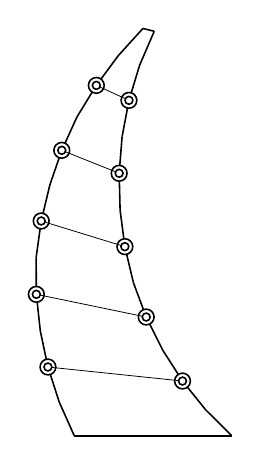
\begin{tikzpicture}
\tikzset{
    scale=2,
    part/.style={line width = .2mm, color=black},
    joint/.style={line width = .2mm, color=black, fill=white},
    grid line/.style={gray},
    link/.style={line width=.1mm, color=black}
    }

\draw[part] (-1.250000, 0.000000) coordinate(Llast) -- (-0.250000, 0.000000) coordinate(Rlast);

\path (-1.345226, 0.213695) coordinate(L) -- (-0.415867, 0.164991) coordinate(R);
\draw[part] (L)--(Llast) (R)--(Rlast);
\path (L)coordinate(Llast) (R)coordinate(Rlast);
\path (-1.417054, 0.436349) coordinate(L) -- (-0.562515, 0.347276) coordinate(R);
\draw[part] (L)--(Llast) (R)--(Rlast);
\path (L)coordinate(Llast) (R)coordinate(Rlast);
\path (-1.465401, 0.665251) coordinate(L) -- (-0.688593, 0.544350) coordinate(R);
\draw[part] (L)--(Llast) (R)--(Rlast);

\draw[joint] (Llast)circle(.05);
\draw[joint] (Rlast)circle(.05);
\draw[link] (Llast)--(Rlast);
\draw[joint] (Llast)circle(.025);
\draw[joint] (Rlast)circle(.025);
\path (L)coordinate(Llast) (R)coordinate(Rlast);
\path (-1.490682, 0.897834) coordinate(L) -- (-0.793126, 0.753650) coordinate(R);
\draw[part] (L)--(Llast) (R)--(Rlast);
\path (L)coordinate(Llast) (R)coordinate(Rlast);
\path (-1.491884, 1.131783) coordinate(L) -- (-0.874552, 0.972975) coordinate(R);
\draw[part] (L)--(Llast) (R)--(Rlast);

\draw[joint] (Llast)circle(.05);
\draw[joint] (Rlast)circle(.05);
\draw[link] (Llast)--(Rlast);
\draw[joint] (Llast)circle(.025);
\draw[joint] (Rlast)circle(.025);
\path (L)coordinate(Llast) (R)coordinate(Rlast);
\path (-1.459694, 1.363510) coordinate(L) -- (-0.928553, 1.200610) coordinate(R);
\draw[part] (L)--(Llast) (R)--(Rlast);
\path (L)coordinate(Llast) (R)coordinate(Rlast);
\path (-1.405224, 1.591033) coordinate(L) -- (-0.958754, 1.432605) coordinate(R);
\draw[part] (L)--(Llast) (R)--(Rlast);

\draw[joint] (Llast)circle(.05);
\draw[joint] (Rlast)circle(.05);
\draw[link] (Llast)--(Rlast);
\draw[joint] (Llast)circle(.025);
\draw[joint] (Rlast)circle(.025);
\path (L)coordinate(Llast) (R)coordinate(Rlast);
\path (-1.329166, 1.812277) coordinate(L) -- (-0.964684, 1.666482) coordinate(R);
\draw[part] (L)--(Llast) (R)--(Rlast);
\path (L)coordinate(Llast) (R)coordinate(Rlast);
\path (-1.232102, 2.025144) coordinate(L) -- (-0.945956, 1.899684) coordinate(R);
\draw[part] (L)--(Llast) (R)--(Rlast);

\draw[joint] (Llast)circle(.05);
\draw[joint] (Rlast)circle(.05);
\draw[link] (Llast)--(Rlast);
\draw[joint] (Llast)circle(.025);
\draw[joint] (Rlast)circle(.025);
\path (L)coordinate(Llast) (R)coordinate(Rlast);
\path (-1.109839, 2.224607) coordinate(L) -- (-0.902571, 2.129578) coordinate(R);
\draw[part] (L)--(Llast) (R)--(Rlast);
\path (L)coordinate(Llast) (R)coordinate(Rlast);
\path (-0.970825, 2.412780) coordinate(L) -- (-0.834465, 2.353398) coordinate(R);
\draw[part] (L)--(Llast) (R)--(Rlast);

\draw[joint] (Llast)circle(.05);
\draw[joint] (Rlast)circle(.05);
\draw[link] (Llast)--(Rlast);
\draw[joint] (Llast)circle(.025);
\draw[joint] (Rlast)circle(.025);
\path (L)coordinate(Llast) (R)coordinate(Rlast);
\path (-0.813637, 2.586058) coordinate(L) -- (-0.741974, 2.568291) coordinate(R);
\draw[part] (L)--(Llast) (R)--(Rlast);
\path (L)coordinate(Llast) (R)coordinate(Rlast);
\draw[part] (L)--(R);
\end{tikzpicture}
\end{document}
